

% Ensuring data integrity is fundamental to secure communication. Without integrity check mechanisms, receivers cannot verify the authenticity of received data, leaving systems vulnerable to malicious data modification. The critical role of integrity verification has been underscored by several real-world incidents. For instance, in 2011, a U.S. drone lacking GPS integrity checks was captured after adversaries successfully hijacked it by transmitting falsified GPS signals (GPS spoofing attack)~\cite{drone_gps_spoofing}.

% To mitigate such vulnerabilities, integrity-check mechanisms are indispensable. In practice, this is most commonly realized through the Message Authentication Code (MAC), computed from the message and a secret key shared between sender and receiver. The tag is transmitted alongside the message, allowing the receiver to verify its integrity. However, generating and transmitting these additional bits introduces both communication and computational overhead, which can be especially costly in power-constrained or latency-sensitive systems.
% % \textcolor{red}{ Leading to many systems, including the Global Navigation Satellite System (GNSS), to avoid implementing integrity check mechanisms~\cite{compoundMAC}}.
% Fifth-generation (5G) network is another case in point, which leaves MAC implementation optional for mobile network operators~\cite {etsi_ts_133501_v17_5_0, 5G_criticality}. However, to reduce security risks, the integrity check implementation should be mandatory. This implies the necessity of research in reducing MAC overhead in order to maintain the performance. 


Ensuring data integrity is fundamental to secure communication. Without integrity checks, receivers cannot verify the authenticity of received data, leaving systems vulnerable to malicious modification. The critical role of integrity verification has been underscored by real-world incidents; for example, in 2011 a U.S.\ drone reportedly lacking GPS integrity checks was captured after adversaries hijacked it by transmitting falsified GPS signals (a GPS spoofing attack)~\cite{drone_gps_spoofing}. In practice, data integrity is most commonly realized via Message Authentication Codes (MACs): a short tag computed from the message using a secret key shared between sender and receiver. Transmitting and verifying MACs, however, introduces both communication and computational overhead, which is especially costly in power-constrained and latency-sensitive systems. Moreover, in the fifth-generation (5G) cellular standard, MAC deployment at certain layers is not mandatory to maintain high performance and is left optional for mobile network operators to implement~\cite{etsi_ts_133501_v17_5_0,5G_criticality}. This further motivates techniques that reduce overhead without compromising security.

% Previous efforts, such as short MAC, aggregate MAC, compound MAC ..., have aimed to decrease this overhead~\cite{ProMAC1, aggregateMAC, compoundMAC}. Nonetheless, these solutions fall short in ensuring data integrity in adversarial environments. Short MAC, as illustrated in Figure~\ref{fig:truncate}, proposes reducing the tag length to decrease the overhead, at the cost of increasing the likelihood of successful forgery~\cite{ProMAC1}. Short MAC's vulnerability was exploited to modify the packets that were transmitted to a badge reader, allowing unauthorized access to a secured building~\cite{badgeOfShame}.
% \begin{figure}[h!]
%     \centering
%     \begin{subfigure}{\columnwidth}
%     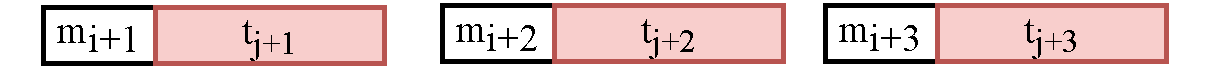
\includegraphics[width= \columnwidth]{img/MAC/TradMAC.pdf} 
%     \caption{Traditional MAC}
%         \vspace{.3cm}
%     \label{fig:traditional}
%     \end{subfigure}

%     \begin{subfigure}{\columnwidth}
%     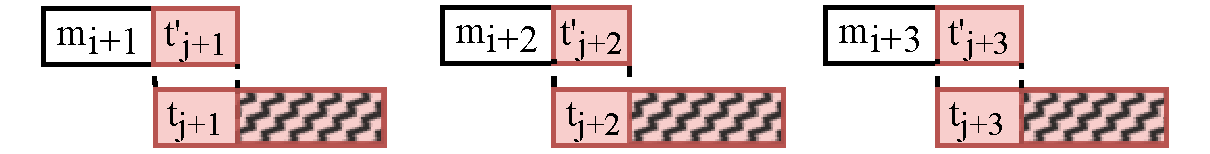
\includegraphics[width= \columnwidth]{img/MAC/TruncMAC.pdf}
%     \caption{Truncate MAC}
%     \label{fig:truncate}
%     \end{subfigure}
%     \caption{\small '$m$' represent the message and '$t$' represents the MAC (also called tag). Truncating the tag decreases the security~\cite{ProMAC1, badgeOfShame}.}
% \end{figure}

% On the other hand, aggregate and compound MACs reduce MAC overhead by verifying a group of multiple messages with only one tag~\cite{aggregateMAC, compoundMAC}. Although this approach could be effective, it is susceptible to random jamming in an adversarial wireless environment. Checking the integrity of multiple messages with one tag creates a verification dependency, where even if one of the dependent messages is lost, the whole group verification will be stopped. This is because the tag requires all of the messages in the group to be correctly received prior to performing the integrity check. Therefore, with even a single message loss, the tag becomes unusable, making the system vulnerable to Denial-of-Service (DoS) attack~\cite{DoS_AggregateMAC, XOR_MAC, proMac2, when_And_How_Aggregate_In_Lossy_Channel}. 

% Among the related works, Progressive MAC (ProMAC) offers a versatile framework that encompasses any MAC aggregation scheme as a system that uses an internal state holding a certain number of messages in the buffer, and an arbitrary update function that updates the internal state of the system after every new message. Then, based on the state of the system, an arbitrary tag generation function will generate and attach a tag to the corresponding message. For example, Figure~\ref{fig:proMAC} shows a system with an internal state of length 3 and a simple update and tag generation function. However, the ProMAC framework lacks guidance on determining optimal configurations, such as the tag generation function and the state update rules. Without a systematic method for adapting these parameters to varying channel conditions, there would be a possibility for security failures.


% This research introduces OptiMAC, a novel optimization framework designed to overcome the limitations of ProMAC in adversarial settings. We have formulated a mathematical model that determines the optimal message-grouping policy to maximize the expected number of usable tags per message under a given message-loss probability. Central to this approach is a graph-based mapping technique that systematically captures the dependencies between messages and tags, enabling the optimization of tag-to-message assignments. By optimizing these assignments, OptiMAC mitigates the vulnerabilities of conventional aggregate and compound MAC schemes, which are prone to random jamming attacks~\cite{when_And_How_Aggregate_In_Lossy_Channel, DoS_AggregateMAC}. The proposed dependency-graph model not only formalizes tag assignment but also provides a mathematical framework for deriving optimal solutions.

% % For an environment with a high packet loss probability, due to random jamming, we have maximized the number of tags that, on average, verify a message.

% While other related schemes rely on heuristic or fixed message-to-tag configurations, OptiMAC can dynamically determines optimal assignments that adapt to varying channel conditions. Our proposed solution not only provides a mathematical framework for optimization but also, through our proposed metrics, can be a basis for analyzing any MAC aggregation schemes in adversarial environments. The OptiMAC is evaluated in a real-world Wi-Fi and 5G testbed. OptiMAC demonstrated a significant improvement in security by increasing the number of usable tag per message for adversarial conditions. This improvement comes with minimal impact on overhead, making it a practical solution for environments where security and efficiency must be carefully balanced.
























Prior attempts to cut overhead follow two main directions. The first is to shorten the tag itself (``short MAC,'' Fig.~\ref{fig:truncate}). While this immediately saves bits, it also lowers the difficulty of successful forgery~\cite{ProMAC1}; in fact, short MACs have been abused in practice to modify packets accepted by a badge reader and gain unauthorized access~\cite{badgeOfShame}. 
\begin{figure}
    \centering
    \begin{subfigure}{\columnwidth}
    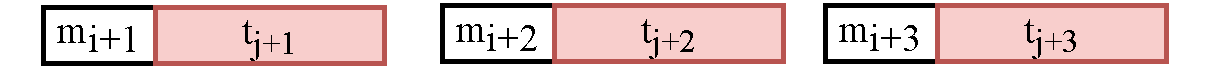
\includegraphics[width= \columnwidth]{img/MAC/TradMAC.pdf} 
    \caption{Traditional MAC}
        \vspace{.3cm}
    \label{fig:traditional}
    \end{subfigure}

    \begin{subfigure}{\columnwidth}
    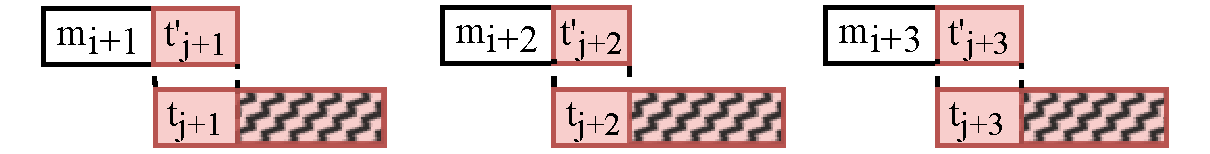
\includegraphics[width= \columnwidth]{img/MAC/TruncMAC.pdf}
    \caption{Truncate MAC}
    \label{fig:truncate}
    \end{subfigure}
    \caption{\small '$m_i$' represent the message and '$t_j$' represents the MAC (also called tag). Truncating the tag decreases the security~\cite{ProMAC1, badgeOfShame}.}
\end{figure}
The second direction is to use one tag across multiple messages using aggregate MAC or aggregate message techniques~\cite{aggregateMAC,compoundMAC, compundMAC_original}. Nonetheless, aggregating creates verification dependencies: the tag can only verify the integrity of the group if all of its dependent messages arrive correctly. In lossy or adversarial wireless settings (e.g., under jamming), losing even a single dependent message makes the tag unusable and enables denial-of-service against the integrity check~\cite{DoS_AggregateMAC,XOR_MAC,proMac2,when_And_How_Aggregate_In_Lossy_Channel}.

\begin{table*}[h]
	\centering
	\caption{Prior approaches vs.\ OptiMAC (qualitative comparison).}
	\label{tab:rw-compare}
	% \begin{tabular}{p{2.8cm}p{3.7cm}p{2.1cm}p{2cm}p{2.6cm}p{1.8cm}}
		\begin{tabular}{llllll}
			\toprule
			\textbf{Approach} & \textbf{Overhead handling} & \makecell[l]{\textbf{Jamming}\\ \textbf{resistance}} & \makecell[l]{\textbf{\# tag assigned} \\ \textbf{per~msg}} & \textbf{\# tag (n) vs. \# msg (m)} & \textbf{Tag size} \\
			\midrule
			Traditional MAC & None & Highest  & 1 (fixed) &$n=m$ (fixed) & High\\
			Short MAC~\cite{badgeOfShame} & Tag truncation & Highest &1 (fixed) & $n=m$ (fixed)& Low\\
			Agg. MAC~\cite{aggregateMAC,sequential_aggregate} & Grouping & Low &1 (fixed)&  $n\leq m$ (semi-flexible)& High\\
			Agg. msg~\cite{compundMAC_original,compoundMAC} & Grouping & Low &1 (fixed)&  $n\leq m$ (semi-flexible)& High\\
			ProMACs~\cite{ProMAC1, cuMAC} & \makecell[l]{Stateful multi-verification} & Low & $\geq 1$ (flexible)& $n=m$ (fixed) & Low\\
			SP-MAC~\cite{proMac2} & \makecell[l]{Golomb rulers based \\dependency assignment} & Medium & $\geq 1$ (flexible)& $n=m$ (fixed) & Low\\ 
			\textbf{OptiMAC} & \textbf{Optimizing dependencies} & \textbf{High} & \textbf{Optimized} &  $n\leq m$ \textbf{(fully flexible)} & \textbf{Optima} \\
			\bottomrule
		\end{tabular}
	\end{table*}


Armknecht et al.~\cite{ProMAC1} proposed the Progressive MAC (ProMAC) framework, which generalizes many aggregation schemes by maintaining an internal state (a buffer) that is updated with each new message and then used to generate tags. A notable realization of this framework, the Whips scheme, cross-assigns tags across multiple messages so that each message is verified several times. This allows shorter tags to achieve the same effective security level as a longer tag can provide in a traditional MAC~\cite{ProMAC1}. However, like aggregate MAC, Whips was designed for error-free channels. In practice, on jammed or lossy wireless links, Whip is susceptible to sandwich attack~\cite{proMac2}. In adversarial settings, an integrity-check scheme must therefore explicitly account for message loss and maximize goodput, which jointly accounts for the amount of message bits that is integrity verified and the total transmitted tag bits. Intuitively, goodput improves when tag overhead is reduced while ensuring that a equal or higher number of message bits remain verifiable. Directly optimizing this trade-off, however, is extremely challenging.

% : it requires simultaneously assigning tags to messages, evaluating the probability that each tag remains usable under loss and jamming, and selecting tag lengths that jointly influence both the numerator and denominator of the goodput expression. These interdependent decisions form a tightly coupled, combinatorial, and highly non-convex problem, rendering a single unified optimization approach exceedingly difficult.

To solve this problem, our proposed OptiMAC approach follows a divide-and-conquer strategy to improve the goodput by first maximizing the expected number of tag verification and second finding the optimal tag length. 

% Optimizing tag size according to the loss probability is important. Arbitrarily shortening tags could reduce the number of messages that satisfy security requirements and thus harm goodput; by first increasing the likelihood that each message is verified multiple times by different tags and only then truncating tag length within the security constraints, OptiMAC improves goodput without hindering the number of messages the receiver can verify.

% We evaluate OptiMAC on live UDP webcam streams over Wi-Fi and 5G, comparing against trad. MAC, aggregate MAC, and ProMAC baselines. Across a range of loss and jamming conditions, OptiMAC increases the realized verifications per message, therefore delivers higher or least similar goodput compared to existing methods. The gains come from aligning tag-to-message assignment with the channel condition first, and only then tuning tag length accordingly to the satisfy the security requirement.

\subsection*{Summery of contributions}

\textbf{Flexible integrity-check framework.} We propose OptiMAC, an extension of the Progressive MAC (ProMAC) framework, to enable applications to choose flexible arbitrary tag-to-message ratios and fine-tune the balance between integrity overhead and security.

\textbf{Optimization-based tag assignment.} We designed a novel optimization model that systematically assigns tags to messages so as to maximize the expected number of usable tags under packet loss and jamming. 

\textbf{Precomputed methods for online adaptation.}
OptiMAC enables applications to precompute optimal configurations for a range of channel conditions and then adapt to the appropriate configuration during online operation.


\textbf{Comprehensive evaluation.} Through large-scale simulations and real-world live UDP webcam streams over Wi-Fi and 5G, we evaluated OptiMAC Across a range of loss and jamming conditions. We demonstrate that OptiMAC achieves superior goodput while maintaining a $256$-bit security level, in particular, under periodic jamming.




Overall, OptiMAC unifies security, efficiency, resilience, and flexibility in a single framework, offering a practical and theoretically sound solution to integrity verification in lossy and adversarial communication environments.






